\documentclass[pdflatex,sn-mathphys-num]{sn-jnl}

\usepackage[utf8]{inputenc}
\usepackage[T1]{fontenc}
\usepackage{lmodern}
\usepackage{graphicx}
\usepackage{multirow}
\usepackage{amsmath,amssymb,amsfonts}
\usepackage{amsthm}
\usepackage{mathrsfs}
\usepackage[title]{appendix}
\usepackage{xcolor}
\usepackage{textcomp}
\usepackage{manyfoot}
\usepackage{booktabs}
\usepackage{algorithm}
\usepackage{algorithmicx}
\usepackage{algpseudocode}
\usepackage{listings}

\raggedbottom

\theoremstyle{thmstyleone}
\newtheorem{proposition}{Proposición}

\begin{document}

\title[Perfil estacional con pesos jerárquicos para el pronóstico de ventas minoristas]{Pronóstico mensual de ventas minoristas por categoría y región con un perfil estacional de pesos jerárquicos: una comparación registrada frente a ocho modelos de aprendizaje automático en Sample Superstore y tres conjuntos adicionales}

\author[1]{\fnm{Alex} \sur{Teran}}

\affil[1]{\orgname{Universidad del Norte}, \orgaddress{\city{Barranquilla}, \country{Colombia}}}

\abstract{La planificación comercial de una cadena minorista requiere pronósticos mensuales de ventas por categoría y región, pero a ese nivel las series son cortas, ruidosas y de escalas distintas. Sobre el conjunto público Sample Superstore (9{,}994 líneas de pedido, 2014--2017), agregado en 12 series de 48 meses, se propone un perfil estacional con pesos jerárquicos: un modelo que predice un índice de ventas libre de escala combinando un perfil estacional común, estimado con todas las series, con el rezago anual de cada serie mediante un peso por serie que se aprende por descenso por bloques con agrupamiento parcial. Se demuestra que el algoritmo converge al mínimo de su objetivo. Antes de experimentar se registró un protocolo que fija hipótesis, métricas, pruebas y regla de decisión. El modelo se comparó con ocho regresores (KNN, Ridge, Lasso, regresión bayesiana, árbol de decisión, Random Forest, XGBoost y SVR), cada uno ajustado con cuatro métodos de optimización, y con el ingenuo estacional, Theta y HistGradientBoosting, pronosticando 24 meses con validación anidada. Obtuvo el menor error absoluto medio, 2{,}310 USD por serie y mes frente a 2{,}366 de SVR, con un modelo de 25 parámetros y un kilobyte; pero la diferencia no es significativa (Diebold--Mariano $p=0.63$, $d=-0.10$; probabilidad posterior de ser mejor, 0.53), su ventaja proviene de 2016 y no se repite en tres conjuntos adicionales del repositorio de Monash, donde queda tercero, décimo y undécimo de doce. Según la regla registrada, el modelo no es superior.}

\keywords{Pronóstico de ventas minoristas, Perfil estacional, Agrupamiento parcial, Validación anidada, Protocolo registrado, Model Confidence Set}

\maketitle

\section{Introducción}\label{sec:intro}

Pronosticar las ventas es un insumo directo de la planificación minorista: de la cifra esperada dependen las metas de cada región, las compras de inventario de cada categoría y el presupuesto de ingresos del año siguiente \cite{fildes2022}. Esas decisiones no se toman sobre el total de la empresa sino sobre combinaciones de producto y territorio, y a ese nivel las series son más cortas, más ruidosas y de tamaños muy distintos entre sí, lo que dificulta tanto el ajuste de un modelo como la comparación honesta entre varios \cite{fildes2022,hyndman2021}.

La práctica habitual en empresas pequeñas y medianas es proyectar ``lo mismo que el mismo mes del año anterior''. Este pronóstico ingenuo estacional captura la estacionalidad sin estimar parámetros y es la referencia mínima que cualquier método debe superar \cite{hyndman2021}, pero arrastra el ruido de un único mes. Los modelos de aprendizaje automático ofrecen una alternativa: en competencias recientes con ventas minoristas, los ensambles de árboles entrenados sobre muchas series a la vez dominan a los métodos que ajustan cada serie por separado \cite{makridakis2022}, y la teoría de los modelos globales explica por qué: compartir parámetros entre series aumenta el tamaño efectivo de la muestra \cite{monteromanso2021}.

Con pocas series y pocos años aparecen tres problemas. Primero, con tres observaciones de cada mes del año por serie, la estacionalidad individual se estima con mucho ruido, y los ensambles tienen que aprenderla con cientos de parámetros \cite{breiman2001,chen2016}. Segundo, la literatura de pronóstico de demanda propone desde hace décadas estimar la estacionalidad con grupos de series \cite{bunn1993,bunn1999} y contraer los índices individuales \cite{miller2003,chen2007,chen2008,zhang2013}, pero esos métodos eligen una opción por serie o derivan los pesos de fórmulas del error de los índices, no del error de pronóstico. Tercero, con pocos meses de evaluación las diferencias entre modelos suelen ser menores que su variabilidad, y sin pruebas de capacidad predictiva \cite{diebold1995,giacomini2006,hansen2011} ni un protocolo fijado de antemano es fácil atribuir al modelo lo que es azar de la partición \cite{cerqueira2020}.

Este trabajo aborda el problema sobre el conjunto público Sample Superstore \cite{superstore}, que registra las ventas de una cadena minorista de Estados Unidos entre 2014 y 2017 en tres categorías y cuatro regiones. Las contribuciones son cuatro. (i) Un \emph{perfil estacional con pesos jerárquicos}: un perfil común de doce valores, estimado con todas las series sobre un índice libre de escala, que cada serie corrige con su propio rezago anual mediante un peso que se aprende con agrupamiento parcial; se derivan sus reglas de actualización y se demuestra su convergencia. (ii) Una comparación con ocho modelos del aprendizaje supervisado, cada uno ajustado con cuatro métodos de optimización de hiperparámetros (32 combinaciones), y con tres referencias adicionales, mediante validación anidada de origen móvil. (iii) Una validación estadística registrada antes de experimentar: Model Confidence Set, Giacomini--White, Diebold--Mariano y Wilcoxon con corrección de Holm, tamaños de efecto y tres conjuntos de datos adicionales, complementada con una prueba bayesiana con región de equivalencia práctica. (iv) Una evaluación de robustez frente a ruido, menos datos, semillas e incertidumbre de predicción.

La hipótesis registrada es que el modelo propuesto tiene menor error absoluto medio que todas las referencias en Sample Superstore y que lo mantiene en al menos dos de tres conjuntos adicionales. El resultado es mixto y así se reporta: el modelo obtiene el menor error en el conjunto principal, con una fracción del costo de los ensambles, pero la ventaja no es estadísticamente significativa y no se repite fuera de él.

\section{Metodología}\label{sec:metodologia}

\subsection{Formulación del problema y notación}\label{subsec:formulacion}

Sea $y_{s,t}\ge 0$ la venta en dólares (USD) de la serie $s\in\{1,\dots,S\}$, una combinación de categoría y región, en el mes $t\in\{1,\dots,T\}$, con $S=12$ y $T=48$. Se define el nivel reciente de la serie y su índice de ventas como
\begin{equation}
\ell_{s,t}=\frac{1}{12}\sum_{j=1}^{12}y_{s,t-j},\qquad z_{s,t}=\frac{y_{s,t}}{\ell_{s,t}},
\label{eq:indice}
\end{equation}
de modo que $z_{s,t}=1.3$ significa vender 30\% más que el promedio de los doce meses previos. La tarea es aprender una función $f:\mathcal{X}\to\mathbb{R}_{\ge 0}$ que prediga el índice a partir de un vector $\mathbf{x}_{s,t}$ construido únicamente con información disponible antes de iniciar el mes $t$:
\begin{equation}
\mathbf{x}_{s,t}=\Bigl(c_s,\;r_s,\;\tfrac{y_{s,t-12}}{\ell_{s,t}},\;\tfrac{y_{s,t-1}}{\ell_{s,t}},\;\tfrac{1}{3\ell_{s,t}}\textstyle\sum_{j=1}^{3}y_{s,t-j},\;\sin\tfrac{2\pi m_t}{12},\;\cos\tfrac{2\pi m_t}{12}\Bigr),
\label{eq:x}
\end{equation}
donde $c_s$ y $r_s$ son la categoría y la región de la serie y $m_t\in\{1,\dots,12\}$ el mes del año. Los modelos de referencia usan el vector completo; el modelo propuesto solo necesita la serie, $m_t$ y el rezago anual relativo $r^{(12)}_{s,t}=y_{s,t-12}/\ell_{s,t}$. El pronóstico en dólares es
\begin{equation}
\hat{y}_{s,t}=\max\bigl(0,\;\hat{z}_{s,t}\,\ell_{s,t}\bigr).
\label{eq:retorno}
\end{equation}
El criterio para elegir hiperparámetros es el error absoluto medio del índice, $\frac{1}{n}\sum_i|z_i-\hat{z}_i|$, elegido por su robustez ante los valores atípicos que revela el análisis exploratorio; cada algoritmo conserva su función objetivo interna. La Tabla~\ref{tab:notacion} resume la notación.

\begin{table}[!htb]
\caption{Notación utilizada en el artículo.}\label{tab:notacion}
\begin{tabular}{@{}ll@{}}
\toprule
Símbolo & Significado \\
\midrule
$y_{s,t}$, $\hat{y}_{s,t}$ & Venta observada y pronosticada de la serie $s$ en el mes $t$ (USD) \\
$\ell_{s,t}$ & Nivel: promedio de los doce meses anteriores a $t$ (USD) \\
$z_{s,t}$, $\hat{z}_{s,t}$ & Índice de ventas observado y predicho (adimensional) \\
$\mathbf{x}_{s,t}$ & Vector de variables predictoras, Ecuación~\eqref{eq:x} \\
$c_s$, $r_s$, $m_t$ & Categoría, región y mes del año \\
$r^{(12)}_{s,t}$ & Ventas del mismo mes del año anterior relativas al nivel \\
$P_m$ & Perfil estacional común del mes $m$ \\
$w_s$, $w_0$ & Peso del rezago anual de la serie $s$ y peso común \\
$\lambda$ & Fuerza del agrupamiento de los pesos \\
$e_{s,t}$ & Error de pronóstico, $y_{s,t}-\hat{y}_{s,t}$ \\
$d_t$ & Diferencial de pérdida mensual entre dos modelos, Ecuación~\eqref{eq:dt} \\
\botrule
\end{tabular}
\end{table}

\subsection{Descripción del problema y del conjunto de datos}\label{subsec:datos}

\textbf{Descripción general.} Sample Superstore \cite{superstore} es un conjunto de datos público de demostración, descargado de Kaggle y sin licencia formal declarada. Contiene 9{,}994 líneas de pedido y 21 variables (identificadores de pedido, cliente y producto, fechas, modo de envío, segmento, ubicación, categoría, subcategoría, ventas, cantidad, descuento y utilidad) con fechas de pedido entre el 3 de enero de 2014 y el 30 de diciembre de 2017. La variable objetivo, \texttt{Sales}, es continua y no negativa, por lo que la tarea es de regresión.

\textbf{ETL.} \textit{Extracción:} el archivo crudo en formato CSV (codificación Latin-1) se lee desde \texttt{data/raw/}. \textit{Transformación:} las fechas de pedido y de envío se convierten al tipo fecha y las líneas se ordenan cronológicamente; no se encontraron filas duplicadas ni valores faltantes, por lo que no hubo eliminación ni imputación. Las líneas se agregan en ventas totales por categoría, región y mes sobre la rejilla completa de combinaciones, de modo que un mes sin pedidos queda con venta cero en lugar de desaparecer (ocurre en 3 de las 576 celdas). Sobre ese panel se calculan el nivel, el índice y las variables de la Ecuación~\eqref{eq:x}; el primer año de cada serie carece de doce meses de historia y solo aporta rezagos. Para los modelos de referencia, las variables categóricas se codifican \emph{one-hot} y las numéricas se estandarizan dentro de un \texttt{Pipeline}, de manera que las medias y desviaciones se estiman únicamente con los datos de entrenamiento de cada ajuste. \textit{Carga:} el panel final (\texttt{ventas\_mensuales.csv}) tiene $12\times48=576$ filas, de las que 432 (2015--2017) tienen variables completas. Las particiones son siempre temporales, sin mezcla aleatoria, porque barajar meses permitiría al modelo ver el futuro \cite{bergmeir2018,cerqueira2020}; se describen en la Sección~\ref{subsec:evaluacion}. La semilla aleatoria se fija en 42.

\subsubsection{Análisis exploratorio de datos}\label{subsubsec:eda}

La Tabla~\ref{tab:eda} presenta la estadística descriptiva. A nivel de línea de pedido, \texttt{Sales} es fuertemente asimétrica a la derecha (media cuatro veces mayor que la mediana, coeficiente de asimetría 13.0) y el criterio de 1.5 veces el rango intercuartílico marca como atípico el 11.7\% de las líneas; son pedidos reales de alto valor, no errores de captura. La agregación mensual atenúa la asimetría (2.1) pero conserva atípicos, concentrados en Tecnología (Figura~\ref{fig:eda}, derecha).

\begin{table}[!htb]
\caption{Estadística descriptiva de las variables numéricas por línea de pedido, de las ventas mensuales por serie y del índice de ventas. Ninguna variable tiene valores faltantes. Atípicos: observaciones fuera de 1.5 veces el rango intercuartílico.}\label{tab:eda}
\footnotesize
\begin{tabular*}{\textwidth}{@{\extracolsep\fill}lrrrrrrr}
\toprule
Variable & $n$ & Media & Mediana & Desv. est. & Mínimo & Máximo & Atípicos \\
\midrule
\texttt{Sales} (USD) & 9{,}994 & 229.86 & 54.49 & 623.25 & 0.44 & 22{,}638.48 & 1{,}167 \\
\texttt{Quantity} & 9{,}994 & 3.79 & 3.00 & 2.23 & 1.00 & 14.00 & 170 \\
\texttt{Discount} & 9{,}994 & 0.16 & 0.20 & 0.21 & 0.00 & 0.80 & 856 \\
\texttt{Profit} (USD) & 9{,}994 & 28.66 & 8.67 & 234.26 & $-$6{,}599.98 & 8{,}399.98 & 1{,}881 \\
Venta mensual por serie (USD) & 576 & 3{,}988.20 & 3{,}084.80 & 3{,}686.14 & 0.00 & 28{,}546.78 & 39 \\
Índice de ventas $z$ & 432 & 1.12 & 0.89 & 0.92 & 0.00 & 7.19 & 17 \\
\botrule
\end{tabular*}
\end{table}

En el análisis univariado del tiempo, las ventas anuales pasaron de 484{,}248 USD en 2014 y 470{,}532 USD en 2015 a 609{,}206 USD en 2016 y 733{,}215 USD en 2017, es decir, crecimientos de 29.5\% y 20.4\% en los dos últimos años (Figura~\ref{fig:eda}, izquierda). La estacionalidad es marcada: septiembre, noviembre y diciembre concentran el 42.9\% de las ventas, y enero y febrero apenas el 6.7\%. Por factores, Tecnología aporta el 36.4\% de las ventas, Muebles el 32.3\% y Oficina el 31.3\%; por regiones, Oeste 31.6\%, Este 29.5\%, Centro 21.8\% y Sur 17.1\%. La venta mensual media por serie varía entre 2{,}444 USD (Muebles, Sur) y 5{,}520 USD (Tecnología, Este).

En el análisis bivariado, la correlación de Spearman de \texttt{Sales} con la cantidad es 0.33 y con el descuento $-0.06$ a nivel de línea. En el panel, el índice se relaciona con las ventas relativas del mismo mes del año anterior ($\rho=0.33$) y casi nada con las del mes anterior ($\rho=0.07$) o con el promedio de los tres meses previos ($\rho=-0.01$). La Figura~\ref{fig:indice} muestra que el índice sigue un patrón estacional compartido y que la relación con el rezago anual, aunque positiva, es muy dispersa.

El descuento casi no se relaciona con el valor de la venta, pero sí con la utilidad ($\rho=-0.54$): el 13.9\% de las líneas tiene un descuento mayor que 20\% y en conjunto perdió 135{,}376 USD, mientras que el resto de las líneas tiene un margen de 21.8\%, frente a 12.5\% del total. Tres subcategorías pierden dinero (mesas, 17{,}725 USD; libreros, 3{,}473 USD; y suministros, 1{,}189 USD), y Muebles deja un margen de 2.5\%, frente a cerca de 17\% de Tecnología y Oficina. Estos hallazgos no entran en el modelo, que pronostica ventas y no utilidad, pero orientan las recomendaciones de negocio. El análisis exploratorio completo (distribuciones univariadas, relaciones bivariadas, comportamiento en el tiempo, atípicos, mapas por estado y análisis por subcategoría) está en el capítulo de EDA del informe técnico del proyecto, disponible en \url{https://alext09.github.io/SuperstorePython2/}.

\begin{figure}[!htb]
\centering
\includegraphics[width=\linewidth]{figures/eda_overview.pdf}
\caption{Izquierda: ventas mensuales totales de la empresa, con el año que solo aporta historia (2014), la ventana inicial de entrenamiento (2015) y el periodo de evaluación de origen móvil (2016--2017). Derecha: distribución de las ventas mensuales por serie en cada categoría; los puntos son valores atípicos.}
\label{fig:eda}
\end{figure}

\begin{figure}[!htb]
\centering
\includegraphics[width=\linewidth]{figures/eda_index.pdf}
\caption{Izquierda: distribución del índice de ventas por mes del año (2015--2017); la línea discontinua marca el nivel promedio de los doce meses previos. Derecha: índice de ventas frente a las ventas relativas del mismo mes del año anterior; la línea discontinua es la identidad.}
\label{fig:indice}
\end{figure}

\textbf{Decisiones derivadas del análisis exploratorio.} (i) El crecimiento de 2016--2017 y la diferencia de escala entre series motivan el índice de la Ecuación~\eqref{eq:indice}: dividir por el nivel reciente hace comparables las series y elimina la tendencia de la variable objetivo. (ii) Que el patrón estacional del índice sea común a las series motiva estimarlo con todas ellas agrupadas. (iii) Que el rezago anual de una serie sea un predictor ruidoso (un solo mes, con atípicos) motiva no usarlo tal cual, como hace el ingenuo estacional, sino contraerlo hacia el patrón común. (iv) Los atípicos son ventas reales y se conservan; por eso la métrica primaria es el MAE y no el error cuadrático. (v) Descuento, cantidad y utilidad no se conocen antes de que ocurra el mes y se excluyen para evitar fuga de información.

\subsection{Modelos de referencia (baselines)}\label{subsec:sota}

El modelo propuesto se compara con once referencias. Ocho son regresores que predicen el índice $z$ con las variables de la Ecuación~\eqref{eq:x}, dentro de un \texttt{Pipeline} con codificación \emph{one-hot} y estandarización; sea $\mathcal{D}=\{(\mathbf{x}_i,z_i)\}_{i=1}^{n}$ la muestra de entrenamiento ya codificada. \textbf{Ridge} y \textbf{Lasso} ajustan un modelo lineal por mínimos cuadrados con penalización $\ell_2$ y $\ell_1$ \cite{hoerl1970,tibshirani1996}:
\begin{equation}
\hat{\boldsymbol{\beta}}=\arg\min_{\beta_0,\boldsymbol{\beta}}\sum_{i=1}^{n}\bigl(z_i-\beta_0-\mathbf{x}_i^{\top}\boldsymbol{\beta}\bigr)^2+\alpha R(\boldsymbol{\beta}),\qquad R(\boldsymbol{\beta})=\lVert\boldsymbol{\beta}\rVert_2^2\ \text{o}\ \lVert\boldsymbol{\beta}\rVert_1.
\label{eq:ridge}
\end{equation}
La \textbf{regresión bayesiana} \cite{mackay1992} trata los coeficientes como aleatorios, con ruido gaussiano de precisión $\alpha_\varepsilon$ y una previa gaussiana de precisión $\alpha_\beta$ sobre los pesos,
\begin{equation}
z_i\mid\mathbf{x}_i,\boldsymbol{\beta}\sim\mathcal{N}\bigl(\beta_0+\mathbf{x}_i^{\top}\boldsymbol{\beta},\,\alpha_\varepsilon^{-1}\bigr),\qquad \boldsymbol{\beta}\sim\mathcal{N}\bigl(\mathbf{0},\,\alpha_\beta^{-1}\mathbf{I}\bigr),
\label{eq:bayes}
\end{equation}
con previas Gamma sobre $\alpha_\varepsilon$ y $\alpha_\beta$; ambas precisiones se estiman maximizando la evidencia marginal y la predicción es la media posterior, de modo que la penalización de Ridge se aprende de los datos en lugar de fijarse.
\textbf{KNN} promedia el índice de los $k$ vecinos más cercanos, $\hat{f}(\mathbf{x})=\frac{1}{k}\sum_{i\in\mathcal{N}_k(\mathbf{x})}z_i$ \cite{cover1967}. El \textbf{árbol de decisión} particiona el espacio eligiendo en cada nodo la variable $j$ y el umbral $u$ que minimizan la suma de cuadrados de las dos regiones \cite{breiman1984}:
\begin{equation}
\min_{j,u}\Bigl[\sum_{i:\,x_{ij}\le u}\bigl(z_i-\bar{z}_{R_1}\bigr)^2+\sum_{i:\,x_{ij}>u}\bigl(z_i-\bar{z}_{R_2}\bigr)^2\Bigr].
\label{eq:arbol}
\end{equation}
\textbf{Random Forest} promedia 300 árboles crecidos sobre muestras \emph{bootstrap} con subconjuntos aleatorios de variables, $\hat{f}(\mathbf{x})=\frac{1}{B}\sum_{b}T_b(\mathbf{x};\Theta_b)$ \cite{breiman2001}. \textbf{XGBoost} construye 300 árboles aditivos minimizando un objetivo regularizado \cite{chen2016}:
\begin{equation}
\mathcal{L}=\sum_{i=1}^{n}\bigl(z_i-\hat{z}_i\bigr)^2+\sum_{m=1}^{M}\Bigl(\gamma\,T_m+\tfrac{1}{2}\lambda_{\mathrm{x}}\lVert\mathbf{w}_m\rVert_2^2\Bigr).
\label{eq:xgb}
\end{equation}
\textbf{SVR} ajusta $f(\mathbf{x})=\mathbf{w}^{\top}\phi(\mathbf{x})+b$ con núcleo gaussiano bajo la pérdida insensible a $\varepsilon$ \cite{drucker1997}:
\begin{equation}
\min_{\mathbf{w},b}\ \tfrac{1}{2}\lVert\mathbf{w}\rVert_2^2+C\sum_{i=1}^{n}\max\bigl(0,\lvert z_i-f(\mathbf{x}_i)\rvert-\varepsilon\bigr).
\label{eq:svr}
\end{equation}
Las otras tres referencias son el \textbf{ingenuo estacional}, $\hat{y}_{s,t}=y_{s,t-12}$, que representa la práctica actual \cite{hyndman2021}; el método \textbf{Theta} \cite{assimakopoulos2000}, ajustado por serie con desestacionalización multiplicativa, que es la referencia estándar de las competencias de pronóstico; y \textbf{HistGradientBoosting}, el \emph{boosting} por histogramas de la familia de LightGBM \cite{ke2017}. Se usaron scikit-learn 1.7.2 \cite{pedregosa2011}, XGBoost 3.2.0 y statsmodels 0.15.0.

\subsection{Modelo propuesto}\label{subsec:propuesto}

\textbf{Limitación que motiva el diseño.} Con tres observaciones de cada mes del año por serie, la estacionalidad individual es ruidosa: el ingenuo estacional, que usa solo la historia propia, es de las peores referencias, y en todos los modelos de referencia la importancia de las variables se concentra en el mes del año y en el rezago anual. La pregunta es cuánta información tomar del grupo y cuánta de cada serie. La Figura~\ref{fig:metodo} muestra el flujo.

\begin{figure}[!htb]
\centering
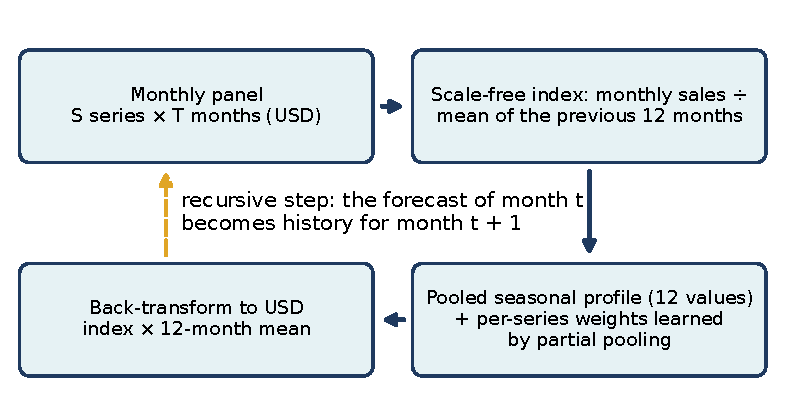
\includegraphics[width=\linewidth]{figures/method_diagram.pdf}
\caption{Flujo del modelo propuesto. El panel en dólares se transforma en un índice libre de escala; el perfil estacional común se estima con todas las series y cada serie lo corrige con un peso aprendido; el resultado se devuelve a dólares. En la proyección a varios meses, cada pronóstico se incorpora a la historia del mes siguiente.}
\label{fig:metodo}
\end{figure}

\textbf{Formulación.} El perfil común es la media del índice en cada mes del año sobre todas las series de entrenamiento, $P_m=\operatorname{media}\{z_{s,t}:m_t=m\}$, y el pronóstico corrige el perfil con el rezago propio:
\begin{equation}
\hat{z}_{s,t}=P_{m_t}+w_s\bigl(r^{(12)}_{s,t}-P_{m_t}\bigr),\qquad 0\le w_s\le 1.
\label{eq:peg}
\end{equation}
Con $w_s=0$ la serie sigue el perfil común y con $w_s=1$ el modelo es el ingenuo estacional. Con $a_{s,t}=z_{s,t}-P_{m_t}$ y $b_{s,t}=r^{(12)}_{s,t}-P_{m_t}$, los pesos y un peso común $w_0$ minimizan
\begin{equation}
J(w_1,\dots,w_S,w_0)=\sum_{s=1}^{S}\sum_{t}\bigl(a_{s,t}-w_s b_{s,t}\bigr)^2+\lambda\sum_{s=1}^{S}\bigl(w_s-w_0\bigr)^2.
\label{eq:objetivo}
\end{equation}
El segundo término acerca cada peso al peso común (agrupamiento parcial): una serie con poca evidencia hereda el peso del grupo. Con $S_{ab,s}=\sum_t a_{s,t}b_{s,t}$ y $S_{bb,s}=\sum_t b_{s,t}^2$, anular la derivada de $J$ respecto de cada bloque da las reglas de actualización
\begin{equation}
w_s\leftarrow\min\Bigl\{1,\max\Bigl\{0,\frac{S_{ab,s}+\lambda w_0}{S_{bb,s}+\lambda}\Bigr\}\Bigr\},\qquad w_0\leftarrow\frac{1}{S}\sum_{s=1}^{S}w_s,
\label{eq:reglas}
\end{equation}
que se alternan hasta que $J$ baja menos de una tolerancia (Algoritmo~\ref{alg:propuesto}). El peso de cada serie promedia su propio peso de mínimos cuadrados, $S_{ab,s}/S_{bb,s}$, y el peso común, según la evidencia $S_{bb,s}$. Para horizontes mayores que uno, las ventas no observadas se sustituyen por sus pronósticos al calcular el nivel y el rezago \cite{taieb2012}.

\begin{algorithm}
\caption{Perfil estacional con pesos jerárquicos}\label{alg:propuesto}
\begin{algorithmic}[1]
\Require Índices $z_{s,t}$, rezagos $r^{(12)}_{s,t}$, meses $m_t$, fuerza $\lambda\ge0$, tolerancia $\tau$
\Ensure Perfil $P_1,\dots,P_{12}$, pesos $w_1,\dots,w_S$ y peso común $w_0$
\State $P_m\gets$ media de $z_{s,t}$ con $m_t=m$, sobre todas las series
\State $a_{s,t}\gets z_{s,t}-P_{m_t}$; \ $b_{s,t}\gets r^{(12)}_{s,t}-P_{m_t}$; \ calcular $S_{ab,s}$ y $S_{bb,s}$
\State $w_0\gets\min\{1,\max\{0,\sum_sS_{ab,s}/\sum_sS_{bb,s}\}\}$; \ $w_s\gets w_0$ para toda $s$
\Repeat
    \State actualizar cada $w_s$ y luego $w_0$ con la Ecuación~\eqref{eq:reglas}
\Until{la disminución de $J$ sea menor que $\tau(1+J)$}
\State \Return $P$, $w$, $w_0$ \Comment{una serie no vista usa $w_0$}
\end{algorithmic}
\end{algorithm}

\begin{proposition}\label{prop:conv}
Si $\lambda>0$ y alguna serie tiene $S_{bb,s}>0$, la sucesión de valores de $J$ no aumenta y el algoritmo converge al único mínimo de la Ecuación~\eqref{eq:objetivo} sobre $[0,1]^S\times\mathbb{R}$.
\end{proposition}

\emph{Demostración.} Con $w_0$ fijo, $J$ es una suma de cuadráticas de una variable con coeficiente principal $S_{bb,s}+\lambda>0$; su mínimo en $[0,1]$ es el mínimo libre recortado, que es la primera regla. Con los $w_s$ fijos, $J$ es cuadrática convexa en $w_0$ y su mínimo es el promedio. Cada paso minimiza $J$ en un bloque, de modo que $J$ no aumenta. La parte cuadrática $\sum_sS_{bb,s}w_s^2+\lambda\sum_s(w_s-w_0)^2$ solo se anula en el origen cuando algún $S_{bb,s}>0$, luego $J$ es estrictamente convexa y tiene un único mínimo; el descenso por bloques con minimización exacta y restricciones separables converge a él \cite{tseng2001}. $\square$

Cuando $\lambda\to\infty$ todas las series comparten un peso, y con $\lambda=0$ cada una usa su peso de mínimos cuadrados. El ajuste cuesta $\mathcal{O}(n+S\,I)$ con $I$ iteraciones, la memoria $\mathcal{O}(S+12)$ y la predicción $\mathcal{O}(1)$ por fila; el modelo entrenado tiene $12+S+1=25$ parámetros y un único hiperparámetro, $\lambda$. La implementación es una clase propia compatible con scikit-learn que solo usa NumPy, con once pruebas unitarias que verifican, entre otras propiedades, el descenso monótono de $J$ y la coincidencia con la solución exacta del sistema lineal de primer orden.

\textbf{Qué es nuevo y qué no.} Estimar la estacionalidad con grupos de series y contraer los índices son ideas conocidas \cite{bunn1993,bunn1999,miller2003,chen2007,chen2008}; el antecedente más cercano combina ambas con pesos derivados de fórmulas del error cuadrático de los índices \cite{zhang2013}. La búsqueda documentada (OpenAlex, Crossref y arXiv, ocho cadenas, noviembre de 2026, con búsqueda por citación) no encontró la regla de la Ecuación~\eqref{eq:reglas}, que aprende un peso por serie a partir del error de pronóstico y agrupa esos pesos, ni su aplicación a este conjunto de datos.

\subsection{Entrenamiento y optimización}\label{subsec:entrenamiento}

Cada uno de los ocho regresores se ajusta con cuatro métodos de optimización de hiperparámetros, 32 combinaciones: búsqueda exhaustiva en rejilla (\emph{grid}), búsqueda aleatoria, optimización bayesiana con Optuna \cite{akiba2019} (modelo sustituto TPE y mejora esperada como función de adquisición \cite{bergstra2011}) y un algoritmo genético con DEAP \cite{fortin2012} (selección por torneo, cruce por mezcla con probabilidad 0.7, mutación gaussiana con probabilidad 0.3 y elitismo de un individuo). Los tres últimos reciben 16 evaluaciones; la rejilla se recorre completa (Tabla~\ref{tab:rejillas}). El modelo propuesto se ajusta igual, con $\lambda\in[0.01,1000]$ en escala logarítmica. El criterio es el error absoluto medio del índice en validación cruzada temporal. El preprocesamiento vive dentro del \texttt{Pipeline} y se ajusta en cada pliegue, y la semilla es 42.

\begin{table}[!htb]
\caption{Espacios de búsqueda. La rejilla se recorre completa; las búsquedas aleatoria, bayesiana y genética exploran los rangos indicados con 16 evaluaciones (escala logarítmica para $\alpha$, $C$, $\gamma$, las previas de la regresión bayesiana, la tasa de aprendizaje y $\lambda$). En la regresión bayesiana la rejilla varía la forma de ambas previas.}\label{tab:rejillas}
\footnotesize
\begin{tabular*}{\textwidth}{@{\extracolsep\fill}p{0.20\textwidth}p{0.60\textwidth}c}
\toprule
Modelo & Hiperparámetros y rangos & Rejilla \\
\midrule
KNN & $k\in[3,30]$; pesos uniformes o por distancia & 12 \\
Ridge & $\alpha\in[0.01,100]$ & 5 \\
Lasso & $\alpha\in[10^{-4},10^{-1}]$ & 4 \\
Regresión bayesiana & forma y tasa de las previas Gamma de $\alpha_\varepsilon$ y $\alpha_\beta$, $\in[10^{-7},10^{-1}]$ & 9 \\
Árbol de decisión & profundidad $\in[2,6]$; mínimo por hoja $\in[1,20]$ & 16 \\
Random Forest & profundidad $\in[2,8]$; mínimo por hoja $\in[1,10]$; fracción de variables $\in[0.4,1]$ & 24 \\
XGBoost & profundidad $\in[2,4]$; tasa $\in[0.02,0.2]$; submuestra $\in[0.7,1]$; peso mínimo de hijo $\in[1,5]$ & 24 \\
SVR & $C\in[0.1,10]$; $\varepsilon\in[0.05,0.2]$; $\gamma\in[0.01,0.3]$ & 18 \\
HistGradientBoosting & tasa $\in[0.02,0.2]$; profundidad $\in[2,4]$; mínimo por hoja $\in[5,20]$ & -- \\
Modelo propuesto & $\lambda\in[0.01,1000]$ & 12 \\
\botrule
\end{tabular*}
\end{table}

\subsection{Protocolo de evaluación}\label{subsec:evaluacion}

\textbf{Protocolo registrado.} Antes de los experimentos definitivos se congeló un documento con las hipótesis, las métricas, los conjuntos adicionales, las particiones, las pruebas, el presupuesto de ajuste y la regla de decisión, marcado con una etiqueta en el repositorio. El conjunto principal ya se había usado para diseñar el modelo en dos iteraciones previas, lo que se declara como limitación; los conjuntos adicionales no se habían usado. \emph{Desviaciones declaradas:} la regresión bayesiana no figuraba en el protocolo; se añadió después, por estar entre los modelos del curso, con exactamente el mismo procedimiento que las demás referencias, y todas las correcciones por multiplicidad y el Model Confidence Set se calculan con ella incluida. El $R^2$, los estadísticos de las pruebas y la prueba bayesiana tampoco estaban registrados: son análisis exploratorios que no entran en la regla de decisión.

\textbf{Validación anidada de origen móvil.} En el bucle externo, cada uno de los 24 meses de 2016 y 2017 se pronostica entrenando con todos los meses anteriores (ventana creciente desde 2015): 288 pronósticos por modelo en 24 bloques mensuales \cite{cerqueira2020}. En el bucle interno, una validación cruzada temporal con pliegues de tres meses (hasta cuatro) elige los hiperparámetros dentro de cada ventana de entrenamiento. Todos los modelos usan las mismas filas y los mismos pliegues. De cada regresor se compara su mejor combinación según el error del bucle externo, lo que favorece a las referencias; del modelo propuesto, la búsqueda bayesiana, fijada en el protocolo.

\textbf{Conjuntos adicionales.} Tres paneles mensuales del repositorio de Monash \cite{godahewa2021}, de naturaleza distinta: turismo (estacionalidad fuerte), hospital (estacionalidad débil) y M3 mensual (series de seis dominios sin estacionalidad común, incluido como caso adverso). De cada uno se tomaron 24 series al azar con los últimos 48 meses completos y se aplicó el mismo protocolo con búsqueda bayesiana.

\textbf{Métricas.} La primaria es el error absoluto medio (MAE) en unidades originales. Las secundarias son la raíz del error cuadrático medio (RMSE), el error porcentual absoluto ponderado (WAPE), el MASE \cite{hyndman2006}, escalado con el error del ingenuo estacional antes del primer origen, el coeficiente de determinación y el desvío del total:
\begin{equation}
\mathrm{WAPE}=\frac{\sum_{s,t}\lvert e_{s,t}\rvert}{\sum_{s,t}y_{s,t}},\qquad
R^2=1-\frac{\sum_{s,t}e_{s,t}^2}{\sum_{s,t}(y_{s,t}-\bar{y})^2},\qquad
\Delta_{\mathrm{total}}=\frac{\sum_{s,t}\hat{y}_{s,t}}{\sum_{s,t}y_{s,t}}-1.
\label{eq:metricas}
\end{equation}
El WAPE sustituye al error porcentual absoluto medio (MAPE) porque hay meses con venta cero, en los que el error porcentual no está definido, y porque el MAPE da el mismo peso a una serie pequeña que a una grande.

\textbf{Pruebas de hipótesis.} Las pruebas usan el diferencial mensual de pérdida absoluta frente a cada referencia $b$, promediado sobre las series para absorber la dependencia entre series de un mismo mes:
\begin{equation}
d_t=\frac{1}{S}\sum_{s=1}^{S}\bigl(\lvert e^{\mathrm{prop}}_{s,t}\rvert-\lvert e^{b}_{s,t}\rvert\bigr),\qquad t=1,\dots,24.
\label{eq:dt}
\end{equation}
(1) El \emph{Model Confidence Set} \cite{hansen2011} parte de todas las combinaciones y elimina las significativamente peores ($\alpha=0.10$, estadístico de rango, \emph{bootstrap} estacionario). (2) La prueba de Giacomini--White \cite{giacomini2006}, válida con modelos reestimados en cada origen, con instrumentos $(1,d_{t-1})$. (3) Diebold--Mariano \cite{diebold1995} con la corrección de Harvey--Leybourne--Newbold \cite{harvey1997}. (4) Wilcoxon de rangos con signo, que no supone normalidad. (5) La prueba $t$ bayesiana correlacionada \cite{corani2015,benavoli2017}, que con una previa no informativa da como posterior de la diferencia media una $t$ de Student con 23 grados de libertad, centrada en $\bar{d}$ y con escala $\sqrt{(1/T+\rho/(1-\rho))\,\widehat{\mathrm{var}}(d_t)}$; se usa $\rho=0$ porque los meses evaluados no se solapan y $d_t$ no muestra autocorrelación, y se interpreta con cautela por la dependencia temporal. Con una región de equivalencia práctica (ROPE) de $\pm1\%$ de la venta media por serie y mes ($\pm47$ USD en Sample Superstore) informa la probabilidad posterior de que el modelo propuesto sea mejor, equivalente o peor. Las pruebas 2 a 4 comparan el modelo propuesto con las once referencias y se ajustan con Holm \cite{holm1979} ($m=11$, $\alpha=0.05$); la prueba 5 no requiere corrección. Cada contraste lleva un intervalo de confianza del 95\% por \emph{bootstrap} estacionario \cite{politis1994} (10{,}000 réplicas, bloque medio de tres meses), la $d$ de Cohen y la delta de Cliff \cite{cliff1993}. Entre conjuntos se aplica Friedman con la corrección de Iman--Davenport. El modelo se declara superior solo si tiene menor MAE que todas las referencias, al menos tres pruebas rechazan la igualdad frente a la mejor, el efecto no es despreciable ($|d|\ge0.2$ o $|\delta|\ge0.147$) y gana en al menos dos de los tres conjuntos adicionales sin ser significativamente peor en ninguno.

\textbf{Robustez e incertidumbre.} Se mide la sensibilidad a $\lambda$, la estabilidad por semilla (diez semillas para Random Forest y XGBoost), el efecto de contaminar la variable objetivo con ruido y atípicos, y el de entrenar con menos meses o menos series. Se construyen intervalos de predicción conformes \cite{angelopoulos2023}, calibrados solo con meses evaluados anteriores, y se verifica su cobertura.

\subsection{Configuración experimental y disponibilidad}\label{subsec:config}

Los experimentos se ejecutaron en un portátil con AMD Ryzen 5 7520U (4 núcleos, 8 hilos), 8 GB de RAM y Windows 11, sin GPU, con Python 3.10.11, scikit-learn 1.7.2, XGBoost 3.2.0, Optuna 5.0.0, DEAP 1.4.4, pandas 2.3.3, NumPy 2.2.6 y statsmodels 0.15.0. Los orígenes se procesaron en paralelo con \texttt{joblib}; la corrida del conjunto principal tardó 115 minutos, y la de la regresión bayesiana en los cuatro conjuntos, menos de un minuto. Los tiempos de ajuste e inferencia se reportan como mediana sobre los 24 orígenes, en un hilo.

\section{Resultados}\label{sec:resultados}

\subsection{Resumen del montaje experimental}\label{subsec:montaje}

Se evalúan el modelo propuesto, las 32 combinaciones de los ocho regresores y tres referencias adicionales sobre 288 pronósticos a un paso en Sample Superstore, y doce modelos sobre 576 pronósticos en cada conjunto adicional, con la semilla 42. La métrica primaria es el MAE; las secundarias, RMSE, WAPE, MASE, $R^2$ y desvío del total. La incertidumbre se mide sobre los 24 bloques mensuales.

\subsection{Desempeño predictivo global}\label{subsec:global}

La Tabla~\ref{tab:resultados} resume el desempeño de la mejor combinación de cada modelo. El modelo propuesto tiene el menor MAE (2{,}310 USD), WAPE y MASE; es el único con MASE inferior a 1, y es segundo en RMSE, a 4 USD de Random Forest, y en $R^2$ (0.205 frente a 0.207). De las seis métricas, gana en tres, es segundo en dos y quinto en el desvío del total. El $R^2$ es bajo en todos los modelos: a nivel de serie y mes las ventas son muy ruidosas, y el error ronda la mitad de la venta. Su ventaja sobre SVR es de 55 USD (2.3\%), sobre Random Forest de 79 USD (3.3\%) y sobre el ingenuo estacional de 417 USD (15.3\%). La ventaja procede de 2016: ese año su MAE es el menor por 126 USD, pero en 2017 SVR lo supera (2{,}444 frente a 2{,}567 USD). En el desvío del total queda en un grupo de modelos entre $-4\%$ y $-7\%$, mientras SVR y el ingenuo estacional subestiman cerca de una quinta parte. La Figura~\ref{fig:box} muestra que la variabilidad entre meses es mucho mayor que las diferencias entre modelos.

\begin{table}[!htb]
\caption{Desempeño en la validación anidada de origen móvil en Sample Superstore (288 pronósticos). Mejor combinación de cada modelo según el MAE. MAE: media $\pm$ desviación estándar sobre los 24 meses. $\Delta_{\mathrm{total}}$: desvío del total del periodo. En negrita el mejor valor de cada columna y subrayado el segundo. $^{\dagger}$ y $^{\ddagger}$: el modelo propuesto es significativamente mejor según Diebold--Mariano y según Wilcoxon, respectivamente, tras la corrección de Holm ($m=11$, $\alpha=0.05$).}\label{tab:resultados}
\scriptsize
\begin{tabular*}{\textwidth}{@{\extracolsep\fill}llrrrrrrrr}
\toprule
Modelo & Optimizador & MAE (USD) & RMSE & WAPE (\%) & MASE & $R^2$ & $\Delta_{\mathrm{total}}$ (\%) & MAE$_{2016}$ & MAE$_{2017}$ \\
\midrule
Modelo propuesto & Bayesiana & \textbf{2{,}310} $\pm$ 852 & \underline{3{,}445} & \textbf{49.6} & \textbf{0.996} & \underline{0.205} & $-5.1$ & \textbf{2{,}053} & \underline{2{,}567} \\
SVR & Rejilla & \underline{2{,}366} $\pm$ 913 & 3{,}531 & \underline{50.8} & \underline{1.020} & 0.166 & $-18.2$ & 2{,}288 & \textbf{2{,}444} \\
Random Forest & Aleatoria & 2{,}390 $\pm$ 774 & \textbf{3{,}441} & 51.3 & 1.030 & \textbf{0.207} & $-4.9$ & \underline{2{,}179} & 2{,}600 \\
KNN & Aleatoria & 2{,}436 $\pm$ 916 & 3{,}466 & 52.3 & 1.050 & 0.196 & $-5.5$ & 2{,}237 & 2{,}636 \\
HistGradientBoosting & Bayesiana & 2{,}439 $\pm$ 777 & 3{,}486 & 52.3 & 1.051 & 0.187 & \underline{$-4.1$} & 2{,}259 & 2{,}619 \\
Árbol de decisión & Bayesiana & 2{,}480 $\pm$ 837 & 3{,}586 & 53.2 & 1.069 & 0.139 & $-6.8$ & 2{,}251 & 2{,}709 \\
XGBoost & Bayesiana & 2{,}481 $\pm$ 796 & 3{,}560 & 53.2 & 1.070 & 0.151 & $-4.8$ & 2{,}249 & 2{,}713 \\
Lasso & Genética & 2{,}501 $\pm$ 858 & 3{,}474 & 53.7 & 1.078 & 0.192 & $-6.1$ & 2{,}306 & 2{,}696 \\
Regresión bayesiana & Rejilla & 2{,}506 $\pm$ 864 & 3{,}507 & 53.8 & 1.080 & 0.177 & $-7.3$ & 2{,}321 & 2{,}690 \\
Ridge & Aleatoria & 2{,}514 $\pm$ 874 & 3{,}509 & 53.9 & 1.084 & 0.176 & $-6.4$ & 2{,}324 & 2{,}705 \\
Ingenuo estacional$^{\dagger\ddagger}$ & -- & 2{,}728 $\pm$ 928 & 4{,}050 & 58.5 & 1.176 & $-0.098$ & $-19.6$ & 2{,}543 & 2{,}912 \\
Theta$^{\dagger\ddagger}$ & -- & 2{,}756 $\pm$ 752 & 3{,}959 & 59.1 & 1.188 & $-0.049$ & $\mathbf{-0.2}$ & 2{,}743 & 2{,}768 \\
\botrule
\end{tabular*}
\end{table}

\begin{figure}[!htb]
\centering
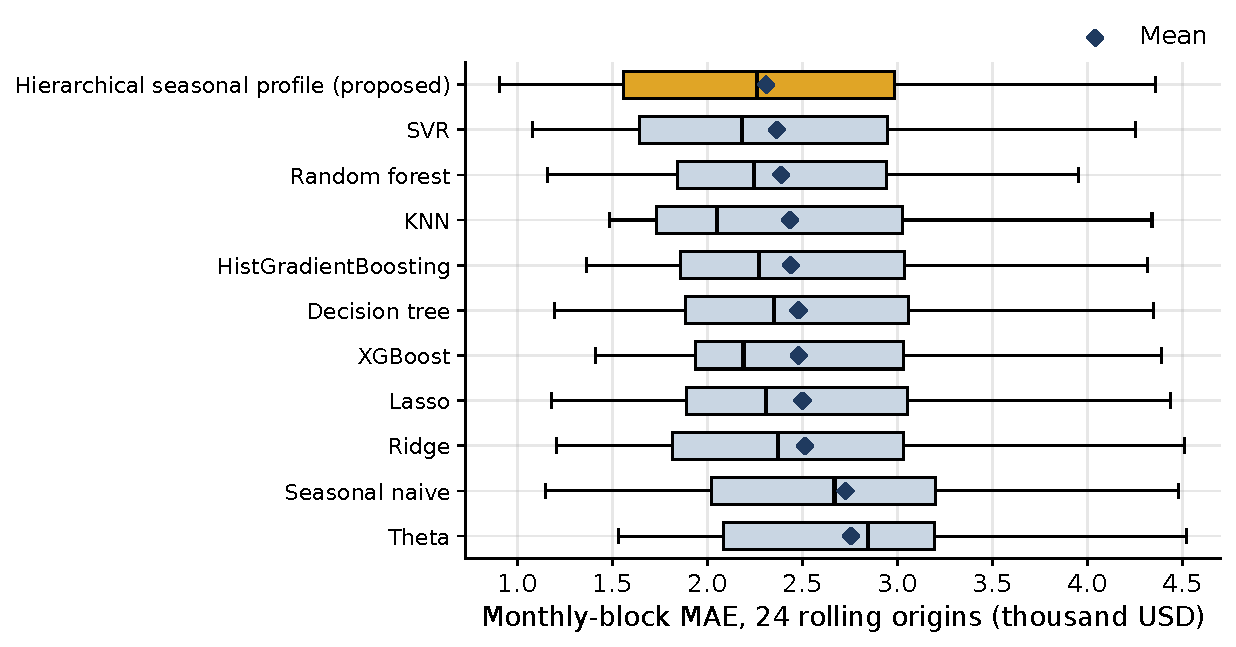
\includegraphics[width=\linewidth]{figures/mae_boxplot.pdf}
\caption{Distribución del MAE de los 24 bloques mensuales de la validación de origen móvil para la mejor combinación de cada modelo. El rombo indica la media.}
\label{fig:box}
\end{figure}

\textbf{Métodos de optimización.} Los cuatro métodos llegan a errores casi iguales: el MAE medio de los nueve modelos ajustados es 2{,}457 USD con la búsqueda bayesiana, 2{,}462 con la rejilla, 2{,}465 con la genética y 2{,}470 con la aleatoria, diferencias mucho menores que la desviación entre meses. La búsqueda genética tarda en promedio 60 s por búsqueda frente a 8.5 s de la bayesiana y 7.8 s de la aleatoria, sin mejorar. Con uno a cuatro hiperparámetros y 16 evaluaciones no hay margen para que los métodos guiados se distingan; el modelo propuesto da prácticamente el mismo error con los cuatro (2{,}309 a 2{,}313 USD).

\begin{figure}[!htb]
\centering
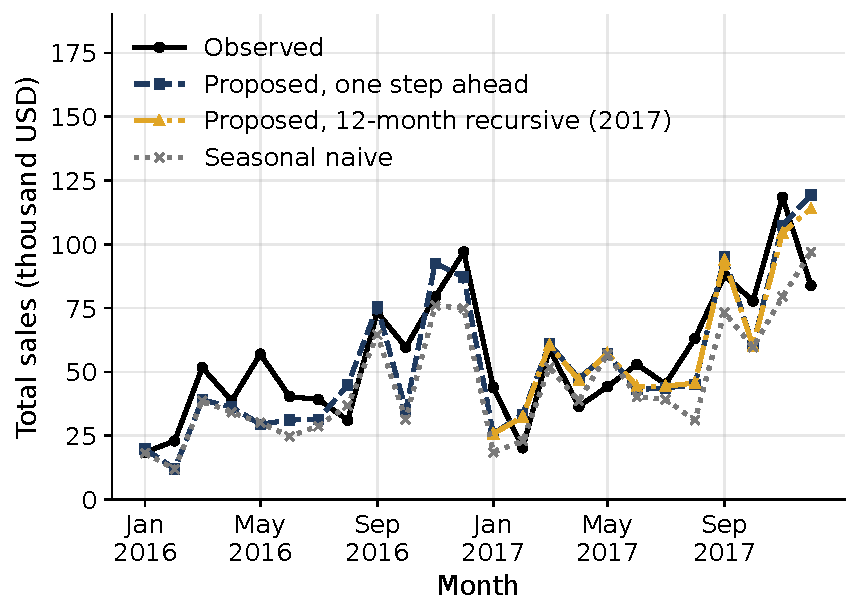
\includegraphics[width=\linewidth]{figures/forecast_total.pdf}
\caption{Ventas totales mensuales de 2016 y 2017: observadas, pronosticadas por el modelo propuesto a un paso, proyectadas de forma recursiva a doce meses para 2017 con datos hasta 2016, y pronóstico ingenuo estacional.}
\label{fig:serie}
\end{figure}

Al agregar las series el error se compensa: proyectando 2017 completo solo con datos hasta 2016, el modelo deja el total anual a $-0.5\%$ del real, con un error típico mensual de 20\% para el total de la empresa (Figura~\ref{fig:serie}).

\subsection{Resultados de las pruebas de significancia}\label{subsec:pruebas}

El Model Confidence Set retiene 34 de las 39 combinaciones, entre ellas el modelo propuesto ($p_{\mathrm{MCS}}=0.48$), SVR y las cuatro de la regresión bayesiana, y solo elimina al ingenuo estacional, a Theta y a tres combinaciones de XGBoost y del árbol de decisión. Con 24 meses, los datos no distinguen a la mayoría de los modelos. Las Tablas~\ref{tab:pruebas} y~\ref{tab:efectos} y la Figura~\ref{fig:dif} presentan los contrastes por pares.

\begin{table}[!htb]
\caption{Pruebas de hipótesis del modelo propuesto frente a cada referencia en Sample Superstore ($T=24$ meses; diferencial $d_t$ de la Ecuación~\eqref{eq:dt}). DM: estadístico de Diebold--Mariano con la corrección de Harvey--Leybourne--Newbold ($t$ con 23 grados de libertad; negativo favorece al propuesto). GW: estadístico de Giacomini--White ($\chi^2_2$). W: estadístico de Wilcoxon de rangos con signo. Para cada prueba, valor $p$ sin ajustar y ajustado por Holm ($m=11$).}\label{tab:pruebas}
\scriptsize
\begin{tabular*}{\textwidth}{@{\extracolsep\fill}lrrrrrrrrr}
\toprule
& \multicolumn{3}{c}{Diebold--Mariano--HLN} & \multicolumn{3}{c}{Giacomini--White} & \multicolumn{3}{c}{Wilcoxon} \\
\cmidrule(lr){2-4}\cmidrule(lr){5-7}\cmidrule(lr){8-10}
Referencia & DM & $p$ & $p_{\mathrm{Holm}}$ & GW & $p$ & $p_{\mathrm{Holm}}$ & W & $p$ & $p_{\mathrm{Holm}}$ \\
\midrule
SVR & $-$0.49 & 0.627 & 0.767 & 0.23 & 0.892 & 1.000 & 101 & 0.169 & 0.675 \\
Random Forest & $-$1.29 & 0.211 & 0.767 & 1.29 & 0.526 & 1.000 & 114 & 0.317 & 0.675 \\
KNN & $-$1.18 & 0.251 & 0.767 & 1.48 & 0.478 & 1.000 & 110 & 0.264 & 0.675 \\
HistGradientBoosting & $-$1.90 & 0.070 & 0.556 & 2.39 & 0.302 & 1.000 & 94 & 0.114 & 0.570 \\
Árbol de decisión & $-$1.66 & 0.110 & 0.767 & 2.08 & 0.354 & 1.000 & 103 & 0.188 & 0.675 \\
XGBoost & $-$2.46 & 0.022 & 0.196 & 4.16 & 0.125 & 1.000 & 75 & 0.031 & 0.233 \\
Lasso & $-$1.51 & 0.145 & 0.767 & 1.93 & 0.380 & 1.000 & 81 & 0.049 & 0.294 \\
Regresión bayesiana & $-$1.59 & 0.124 & 0.767 & 2.06 & 0.357 & 1.000 & 74 & 0.029 & 0.233 \\
Ridge & $-$1.66 & 0.111 & 0.767 & 2.09 & 0.352 & 1.000 & 71 & 0.023 & 0.206 \\
Ingenuo estacional & $-$3.36 & 0.003 & \textbf{0.030} & 7.40 & 0.025 & 0.273 & 51 & 0.004 & \textbf{0.035} \\
Theta & $-$3.22 & 0.004 & \textbf{0.037} & 6.72 & 0.035 & 0.347 & 50 & 0.003 & \textbf{0.035} \\
\botrule
\end{tabular*}
\end{table}

\begin{table}[!htb]
\caption{Tamaño de la diferencia y prueba bayesiana del modelo propuesto frente a cada referencia en Sample Superstore. $\Delta$MAE: diferencia media propuesto menos referencia, en USD, con intervalo del 95\% por \emph{bootstrap} estacionario (negativo favorece al propuesto). $d$: $d$ de Cohen; $\delta$: delta de Cliff. Prueba $t$ bayesiana correlacionada con ROPE de $\pm47$ USD: probabilidad posterior de que el propuesto sea mejor, equivalente o peor. Meses: meses, de 24, en que gana el propuesto.}\label{tab:efectos}
\scriptsize
\begin{tabular*}{\textwidth}{@{\extracolsep\fill}lrrrrrrr}
\toprule
& & & & \multicolumn{3}{c}{Prueba bayesiana} & \\
\cmidrule(lr){5-7}
Referencia & $\Delta$MAE [IC 95\%] & $d$ & $\delta$ & P(mejor) & P(ROPE) & P(peor) & Meses \\
\midrule
SVR & $-$55 [$-$216, 138] & $-$0.10 & 0.00 & 0.53 & 0.28 & 0.19 & 15 \\
Random Forest & $-$79 [$-$168, 10] & $-$0.26 & $-$0.07 & 0.70 & 0.27 & 0.03 & 14 \\
KNN & $-$126 [$-$286, 32] & $-$0.24 & $-$0.07 & 0.77 & 0.17 & 0.06 & 15 \\
HistGradientBoosting & $-$129 [$-$237, $-$18] & $-$0.39 & $-$0.10 & 0.88 & 0.11 & 0.01 & 15 \\
Árbol de decisión & $-$170 [$-$320, $-$14] & $-$0.34 & $-$0.10 & 0.88 & 0.10 & 0.02 & 13 \\
XGBoost & $-$171 [$-$297, $-$55] & $-$0.50 & $-$0.11 & 0.96 & 0.04 & $<$0.01 & 16 \\
Lasso & $-$191 [$-$377, 3] & $-$0.31 & $-$0.12 & 0.87 & 0.10 & 0.04 & 15 \\
Regresión bayesiana & $-$195 [$-$376, $-$6] & $-$0.33 & $-$0.11 & 0.88 & 0.09 & 0.03 & 16 \\
Ridge & $-$204 [$-$382, $-$21] & $-$0.34 & $-$0.13 & 0.89 & 0.08 & 0.03 & 16 \\
Ingenuo estacional & $-$417 [$-$599, $-$211] & $-$0.69 & $-$0.23 & $>$0.99 & $<$0.01 & $<$0.01 & 18 \\
Theta & $-$445 [$-$700, $-$197] & $-$0.66 & $-$0.29 & $>$0.99 & $<$0.01 & $<$0.01 & 19 \\
\botrule
\end{tabular*}
\end{table}

\begin{figure}[!htb]
\centering
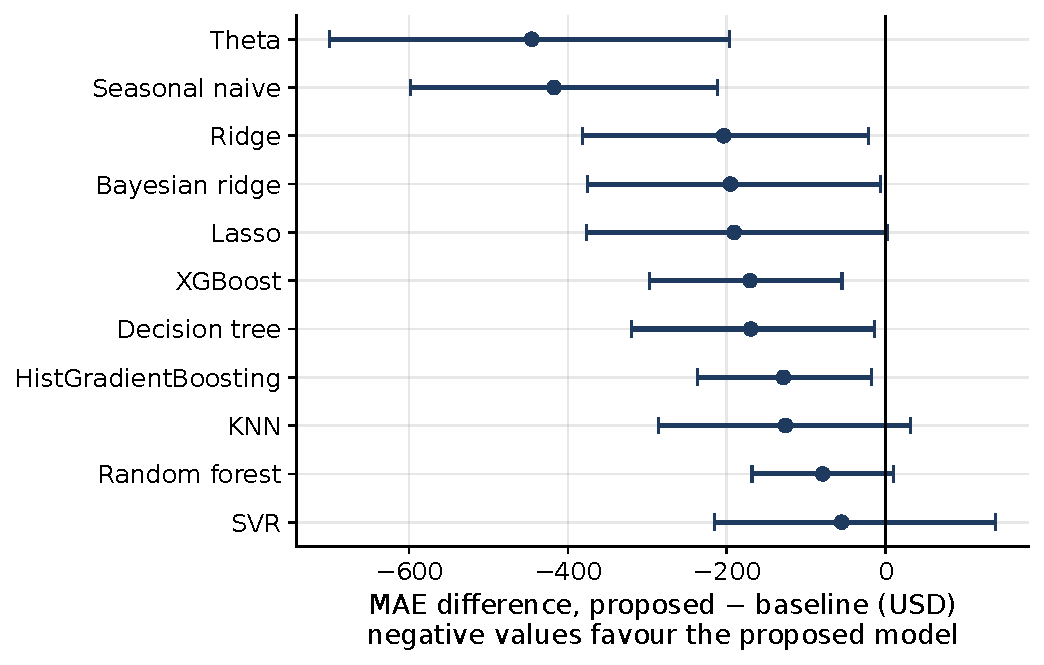
\includegraphics[width=\linewidth]{figures/mae_differences.pdf}
\caption{Diferencia media de MAE entre el modelo propuesto y cada referencia en Sample Superstore, con intervalo de confianza del 95\% por \emph{bootstrap} estacionario.}
\label{fig:dif}
\end{figure}

La diferencia favorece al modelo propuesto en los once contrastes, pero tras la corrección de Holm solo Diebold--Mariano y Wilcoxon rechazan la igualdad, y solo frente al ingenuo estacional y a Theta, con efectos medianos ($d\approx-0.7$): el modelo propuesto supera significativamente a 2 de las 11 referencias y es estadísticamente indistinguible de las otras 9. Giacomini--White no rechaza en ningún caso tras el ajuste. Frente a XGBoost, HistGradientBoosting, Ridge, la regresión bayesiana y el árbol los intervalos excluyen el cero, pero los valores $p$ no sobreviven a once comparaciones. Frente a la mejor referencia, SVR, la diferencia es de 55 USD con un intervalo que contiene al cero, ninguna prueba rechaza y el efecto es despreciable; la prueba bayesiana lo confirma, con probabilidades de 0.53 de que el propuesto sea mejor, 0.28 de equivalencia práctica y 0.19 de que sea peor, es decir, sin evidencia en ningún sentido.

Las pruebas discrepan en un caso. La prueba bayesiana da una probabilidad de 0.96 de que el propuesto supere a XGBoost, mientras Diebold--Mariano y Wilcoxon no rechazan tras Holm; la diferencia se explica porque la probabilidad posterior no se corrige por multiplicidad y porque, con $\rho=0$, no descuenta la dependencia entre meses, que es justamente apreciable en el contraste con XGBoost. Por la misma razón, sus probabilidades de 0.87 a 0.89 frente a los modelos lineales y al árbol son evidencia débil. En términos prácticos, la ventaja sobre SVR equivale al 1.2\% de la venta media por serie y mes (4{,}661 USD), apenas por encima del borde de la región de equivalencia. Las diferencias mensuales no muestran autocorrelación apreciable (Ljung--Box, $p>0.05$ en diez de once casos; la excepción es XGBoost), lo que respalda la estacionariedad que supone Diebold--Mariano y el uso de $\rho=0$; la normalidad se rechaza en seis de once casos (Shapiro--Wilk), de ahí la prueba de Wilcoxon.

\subsection{Conjuntos de datos adicionales}\label{subsec:adicionales}

La Figura~\ref{fig:datasets} resume los cuatro conjuntos. En turismo, de estacionalidad fuerte, el modelo propuesto queda tercero de doce (MASE 0.814), a 5.6 unidades de KNN y sin diferencia significativa (Diebold--Mariano $p_{\mathrm{Holm}}=1.00$); el conjunto de confianza retiene cinco modelos, incluido el propuesto, y descarta a los ensambles de árboles y a los modelos lineales, entre ellos la regresión bayesiana. En hospital, de estacionalidad débil, queda décimo (MASE 0.537 frente a 0.480 de SVR) y los doce modelos son indistinguibles. En M3, cuyas series no comparten estacionalidad, queda undécimo (MASE 0.869) y es significativamente peor que Theta (MASE 0.486; $p_{\mathrm{Holm}}<0.001$). La regresión bayesiana queda séptima en los tres conjuntos adicionales. La prueba de Friedman con la corrección de Iman--Davenport no rechaza que los doce modelos rindan igual en los cuatro conjuntos ($F=0.78$, $p=0.66$); el rango medio del propuesto es 6.25 y el mejor, XGBoost, 4.50. Con cuatro conjuntos la prueba tiene poca potencia, de modo que los resultados por conjunto pesan más que la prueba global.

\begin{figure}[!htb]
\centering
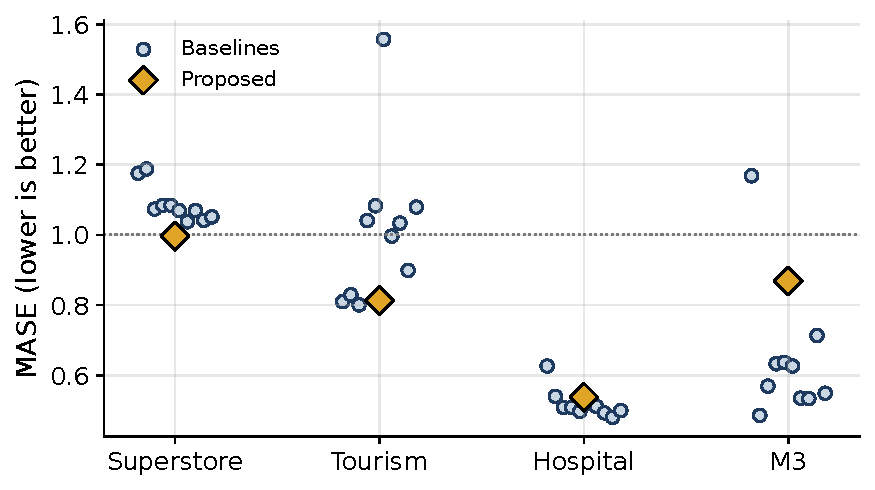
\includegraphics[width=\linewidth]{figures/datasets.pdf}
\caption{MASE de los doce modelos en cada conjunto de datos (búsqueda bayesiana o sin ajuste). El rombo es el modelo propuesto; la línea punteada marca el error del ingenuo estacional de referencia.}
\label{fig:datasets}
\end{figure}

\textbf{Veredicto.} De las cuatro condiciones registradas, el modelo cumple solo la primera: tiene menor MAE que las once referencias en Sample Superstore, pero ninguna prueba rechaza la igualdad frente a SVR, el efecto es despreciable ($d=-0.10$, $\delta=-0.003$) y no gana en ningún conjunto adicional. \textbf{El modelo no es superior.}

\subsection{Sensibilidad y robustez}\label{subsec:sensibilidad}

\textbf{Hiperparámetro.} Con $\lambda$ fijo entre 0.01 y 1000 el MAE varía entre 2{,}280 y 2{,}307 USD, siempre por debajo de SVR (Figura~\ref{fig:sens}, izquierda): el resultado no depende de afinar $\lambda$. El error baja al crecer $\lambda$, es decir, cuando los pesos se acercan a un valor común; la búsqueda elige $\lambda=135$ y pesos entre 0.00 y 0.04. En este conjunto, el peso propio de cada serie aporta poco y lo que funciona es el perfil común.

\begin{figure}[!htb]
\centering
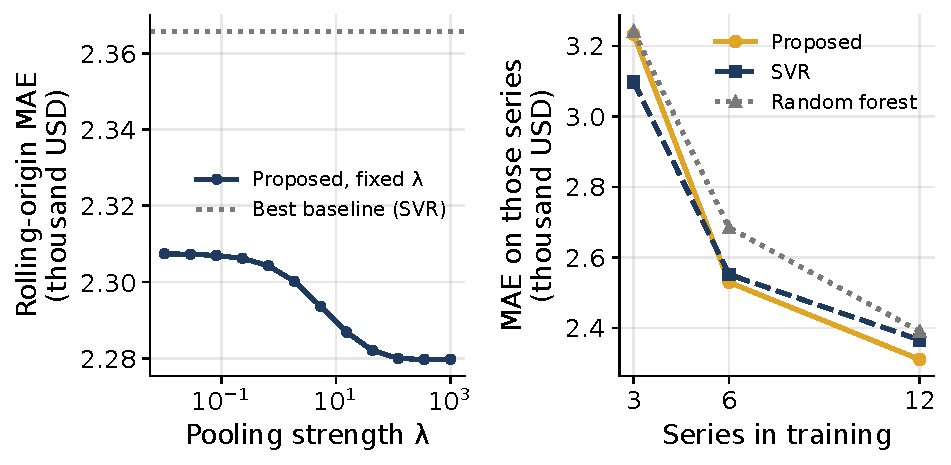
\includegraphics[width=\linewidth]{figures/sensitivity.pdf}
\caption{Izquierda: MAE de origen móvil del modelo propuesto con $\lambda$ fijo; la línea punteada es la mejor referencia. Derecha: MAE al entrenar con 3, 6 y 12 series, para el modelo propuesto y las dos mejores referencias.}
\label{fig:sens}
\end{figure}

\textbf{Menos datos.} Con 12 o 18 meses de entrenamiento el MAE del propuesto sube a 2{,}486 y 2{,}476 USD, como el de las referencias. El número de series le afecta más: con tres series su error (3{,}233 USD) supera al de SVR (3{,}098), porque el perfil común se estima con una cuarta parte de los datos; con seis series ya es el mejor de los tres (Figura~\ref{fig:sens}, derecha).

\textbf{Ruido y atípicos.} Al contaminar la variable objetivo de entrenamiento con ruido multiplicativo de desviación 0.4, el MAE del propuesto cambia menos de 1\% (2{,}325 USD). Un 5\% de atípicos lo eleva a 2{,}424, por encima de SVR (2{,}412), cuya pérdida ignora los errores grandes.

\textbf{Semillas.} El modelo propuesto es determinista. Con diez semillas, Random Forest varía $\pm4$ USD y XGBoost $\pm12$, mucho menos que las diferencias entre modelos.

\textbf{Incertidumbre.} Los intervalos conformes del propuesto cubren el 80.6\% y el 88.2\% de los valores reales con niveles nominales de 80\% y 90\%, con anchos medios de 7{,}302 y 10{,}245 USD, más angostos que los de SVR (8{,}549 y 12{,}123) con cobertura similar. En los conjuntos adicionales la cobertura del propuesto queda a menos de 4 puntos de la nominal.

\subsection{Costo computacional}\label{subsec:costo}

La Tabla~\ref{tab:costo} reúne el costo de cada modelo en el equipo descrito en la Sección~\ref{subsec:config}. El modelo propuesto se ajusta en 4.1 ms y predice el mes en 2.2 ms, frente a 14--22 ms de ajuste de los modelos lineales, KNN, el árbol y SVR, 156 ms de XGBoost, 244 ms de HistGradientBoosting y 741 ms de Random Forest. Guarda 25 números (12 del perfil, 12 pesos y el peso común) y serializado ocupa 1.0 kB, frente a 12{,}016 nodos y 297 kB de Random Forest. Su tiempo de ajuste crece de forma sublineal con el número de filas en el rango medido (exponente empírico 0.75 al replicar los datos hasta 64 veces), consistente con el costo $\mathcal{O}(n)$. Con todos los datos, el algoritmo converge en 21 iteraciones. La mejora en error es pequeña y no significativa frente a SVR o Random Forest, pero llega con uno o dos órdenes de magnitud menos de cómputo y de memoria, y con parámetros que se leen directamente.

\begin{table}[!htb]
\caption{Costo computacional en Sample Superstore, para la mejor combinación de cada modelo. Búsqueda: tiempo medio de la optimización de hiperparámetros por origen. Ajuste e inferencia: mediana sobre los 24 orígenes, en un hilo. Tamaño: modelo final serializado con \texttt{joblib}, usado como medida de la memoria que ocupa. Parámetros: números que el modelo ajustado guarda para predecir (coeficientes, nodos de los árboles, vectores de soporte o, en KNN, el conjunto de entrenamiento). El ingenuo estacional y Theta no se ajustan con búsqueda y no se incluyen.}\label{tab:costo}
\footnotesize
\begin{tabular*}{\textwidth}{@{\extracolsep\fill}lrrrrr}
\toprule
Modelo & Búsqueda (s) & Ajuste (ms) & Inferencia (ms) & Tamaño (kB) & Parámetros \\
\midrule
Modelo propuesto & \textbf{0.8} & \textbf{4.1} & \textbf{2.2} & \textbf{1.0} & 25 \\
SVR & 2.6 & 22.0 & 9.1 & 12.7 & 4{,}265 \\
Random Forest & 48.0 & 741.3 & 32.4 & 296.9 & 12{,}016 \\
KNN & 1.6 & 14.7 & 8.6 & 31.7 & 5{,}616 \\
HistGradientBoosting & 15.5 & 244.5 & 10.6 & 196.4 & 2{,}644 \\
Árbol de decisión & 1.7 & 14.3 & 7.3 & 2.1 & \textbf{7} \\
XGBoost & 9.3 & 156.1 & 9.0 & 30.7 & 1{,}928 \\
Lasso & 1.0 & 14.9 & 7.9 & 1.7 & 13 \\
Regresión bayesiana & 1.1 & 17.6 & 8.8 & 5.2 & 15 \\
Ridge & 1.8 & 14.2 & 7.1 & 1.7 & 13 \\
\botrule
\end{tabular*}
\end{table}

\subsection{Interpretabilidad y análisis de errores}\label{subsec:errores}

\textbf{Interpretación.} Los doce valores del perfil se leen directamente como la estacionalidad del negocio (Figura~\ref{fig:imp}, izquierda): enero y febrero venden 0.64 y 0.55 veces el promedio de los doce meses previos, y septiembre (1.66), noviembre (1.94) y diciembre (1.75) forman la temporada alta. Cada pronóstico se descompone exactamente en la base, el aporte del mes y el aporte del rezago propio; para los modelos de referencia, los valores de Shapley exactos confirman que la predicción depende sobre todo del mes del año y del rezago anual.

\begin{figure}[!htb]
\centering
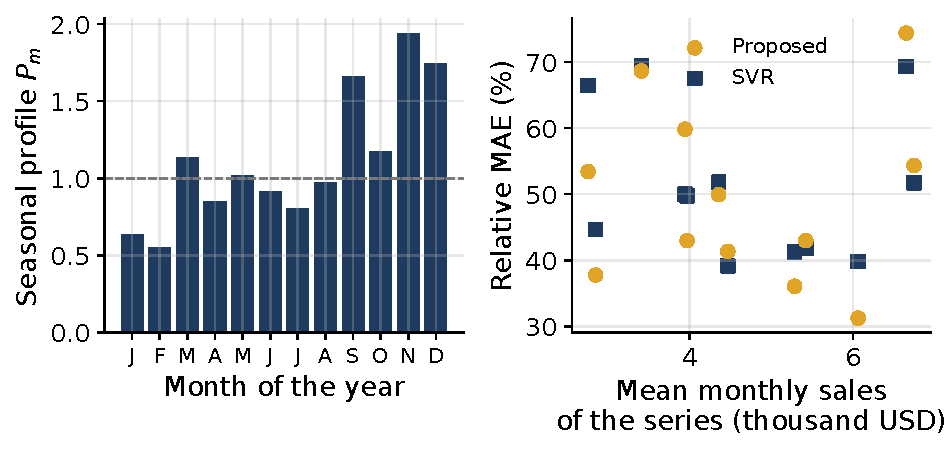
\includegraphics[width=\linewidth]{figures/profile_errors.pdf}
\caption{Izquierda: perfil estacional estimado con 2015--2017; la línea discontinua es el nivel de los doce meses previos. Derecha: MAE relativo a la venta media de cada serie, para el modelo propuesto y SVR.}
\label{fig:imp}
\end{figure}

\textbf{Errores.} El modelo es mejor que SVR en 7 de las 12 series. El error relativo va de 31\% (Muebles, Oeste) a 74\% (Tecnología, Este), y las cuatro series de Tecnología son las de mayor error. Por terciles de venta aparece regresión a la media: sobrestima 1{,}344 USD en el tercil bajo y subestima 2{,}397 en el alto, aunque en ambos su MAE es menor que el de SVR. Los mayores errores son picos de Tecnología no anticipados, como Centro en octubre de 2016 (20{,}370 USD observados frente a 2{,}718 pronosticados). Los residuos son heterocedásticos (White, $p=0.001$) y no muestran autocorrelación (Ljung--Box, $p=0.41$); la Figura~\ref{fig:pred} los resume.

\begin{figure}[!htb]
\centering
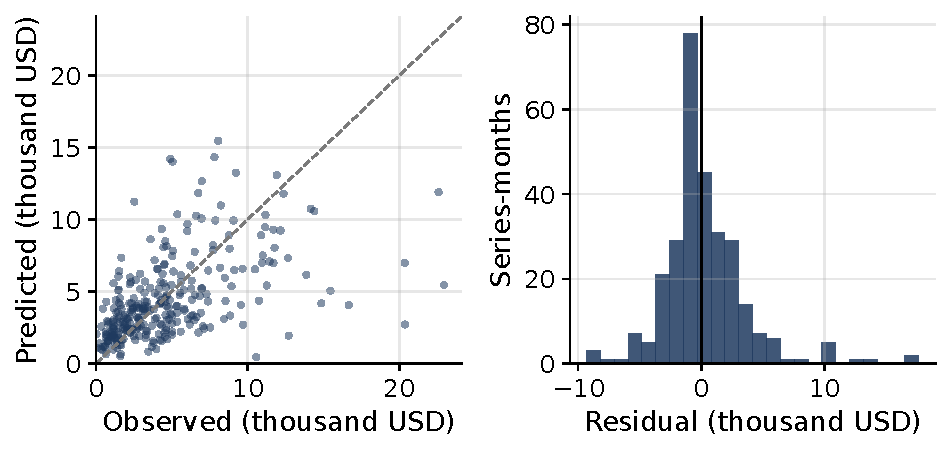
\includegraphics[width=\linewidth]{figures/pred_vs_obs.pdf}
\caption{Modelo propuesto en la validación de origen móvil. Izquierda: ventas pronosticadas frente a observadas por serie y mes; la línea discontinua es la identidad. Derecha: distribución de los residuos.}
\label{fig:pred}
\end{figure}

\subsection{Discusión, limitaciones y amenazas a la validez}\label{subsec:discusion}

\textbf{Discusión.} El resultado dialoga con la literatura en tres puntos. Primero, en un panel de 12 series y 36 meses, la ventaja de los ensambles reportada con miles de series \cite{makridakis2022} no aparece: un modelo de un kilobyte es tan preciso como Random Forest o SVR. Segundo, lo que funciona es compartir la estacionalidad entre series, en línea con el principio de globalidad \cite{monteromanso2021} y con la literatura de índices de grupo \cite{bunn1993,chen2008}; el mecanismo nuevo, el peso por serie, no mejora a un peso único en el conjunto principal, aunque sí en turismo, donde las series difieren más. Tercero, el mismo supuesto que da la ventaja explica el fallo en M3: sin estacionalidad común, el perfil promedia patrones distintos.

\textbf{Limitaciones y amenazas a la validez.} (i) \emph{Diseño informado por los datos:} el modelo se diseñó tras dos iteraciones evaluadas en el conjunto principal; los conjuntos adicionales son la evidencia independiente, y no es favorable. (ii) \emph{Potencia:} 24 meses no permiten detectar diferencias del 1--2\%; la ausencia de significancia no demuestra equivalencia. (iii) \emph{Dependencia del periodo:} la ventaja proviene de 2016. (iv) \emph{Datos de demostración} y muestras de 24 series en los conjuntos adicionales. (v) \emph{Variables:} sin promociones, precios ni calendario comercial, ningún modelo anticipa los pedidos excepcionales. (vi) \emph{Presupuesto desigual en la rejilla:} entre 4 y 24 configuraciones según el modelo, aunque los otros tres métodos usan 16 para todos. (vii) \emph{Fuga de información:} todas las variables usan meses anteriores y toda estimación ocurre dentro de la ventana de entrenamiento. (viii) \emph{Desviaciones del protocolo:} la regresión bayesiana, el $R^2$ y la prueba bayesiana se añadieron después del registro; no cambian el veredicto, pero son análisis posteriores. (ix) \emph{Prueba bayesiana:} supone $\rho=0$ y no se corrige por multiplicidad, por lo que sus probabilidades deben leerse junto con las pruebas frecuentistas.

\section{Conclusiones}\label{sec:conclusiones}

Se propuso un perfil estacional con pesos jerárquicos para pronosticar ventas mensuales por categoría y región, con reglas de actualización derivadas y convergencia demostrada, y se evaluó bajo un protocolo registrado frente a ocho regresores ajustados con cuatro métodos de optimización y tres referencias adicionales. En Sample Superstore obtuvo el menor error absoluto medio (2{,}310 USD por serie y mes), con un modelo de un kilobyte que se ajusta en milisegundos, y supera con significancia al ingenuo estacional y a Theta. Pero la ventaja frente a la mejor referencia, SVR, no es estadísticamente significativa, proviene de 2016 y no se repite en los conjuntos adicionales; según la regla fijada de antemano, el modelo no es superior. Con todos los datos, el modelo proyecta 886{,}866 USD para 2018, 21\% más que 2017.

Como trabajo futuro se propone formar grupos de series con estacionalidad parecida en lugar de un perfil para todo el panel, usar un perfil robusto a los meses atípicos, evaluar con más historia para ganar potencia estadística e incorporar variables de calendario comercial y promociones.

\backmatter

\section*{Declaraciones}

\begin{itemize}
\item \textbf{Disponibilidad de datos:} Sample Superstore es un conjunto de datos público de demostración, descargado de Kaggle \cite{superstore}. Los conjuntos adicionales provienen del repositorio de Monash \cite{godahewa2021}, con licencia CC BY 4.0. Las copias utilizadas y los datos procesados están en el repositorio del proyecto.
\item \textbf{Disponibilidad de código:} el código completo está en \url{https://github.com/AlexT09/SuperstorePython2}. El modelo propuesto está en \texttt{src/original\_model.py}; el protocolo registrado, en \texttt{experiments/protocolo.md}; los experimentos se reproducen con los scripts de \texttt{experiments/} (la regresión bayesiana con \texttt{bayesiana.py} y las tablas de este artículo con \texttt{paper\_tablas.py}) y las figuras con \texttt{paper/figuras.py}. La semilla aleatoria es 42. El tablero interactivo (\url{https://superstorepython2.onrender.com}) y el informe técnico (\url{https://alext09.github.io/SuperstorePython2/}) usan el mismo modelo y los mismos resultados.
\item \textbf{Uso de herramientas de inteligencia artificial:} se usó un asistente de inteligencia artificial para programar el modelo, los experimentos y las pruebas, y para redactar borradores de este artículo; el autor revisó el código y los resultados y es responsable del contenido.
\item \textbf{Contribución del autor:} el autor realizó el diseño del estudio, la implementación, el análisis de resultados y la redacción, y aprobó la versión final.
\item \textbf{Conflicto de intereses:} el autor declara no tener conflictos de interés.
\end{itemize}

\bibliography{sn-bibliography}

\end{document}
